\begin{problem}{Path Sums}{standard input}{standard output}{0.5 seconds}{256 megabytes}

You are given a rooted binary tree with $n$ nodes (that is, each node has at most 2 children). Each node has a value attached to it. Given a query $k$, you are asked to count the number of simple paths whose values sum to exactly $k$.

For simplicity, we will consider a path to be valid in this context if it starts at some node and only moves down the tree. A path is not required to start at the root nor end at a leaf. For example, consider the following binary tree.

\begin{center}
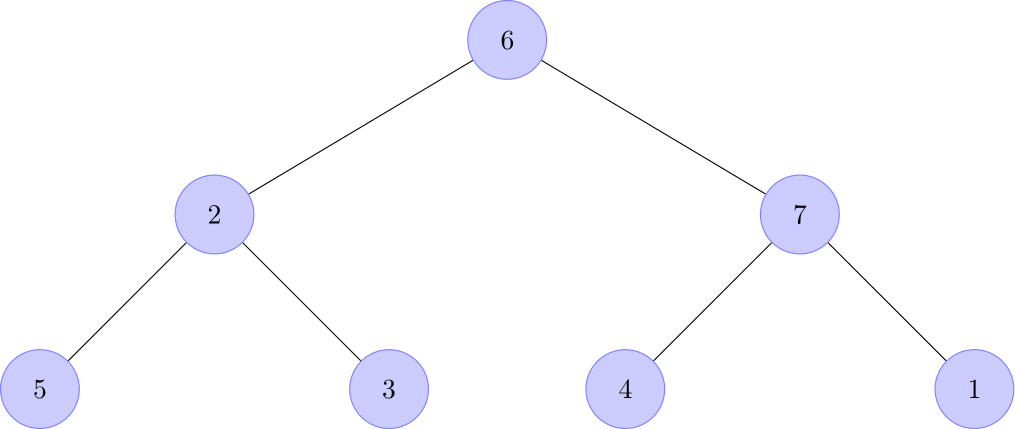
\includegraphics{example_binary_tree.png}
\end{center}

\textbf{6-2-3} would be considered a valid path, as would \textbf{6-7}, \textbf{2-5}, and even \textbf{4}. However, \textbf{4-7-1} is not a valid path because it goes up and then down. Nor would any paths which double back on themselves like \textbf{6-7-1-7}. We are also not considering the empty path to be valid.

\InputFile
The first line contains a single integer $n$, the number of nodes in the tree. Let's call the nodes $v_0, v_1, \dots, v_{n-1}$. $v_0$ is guaranteed to be the root of the tree.

The next $n$ lines $L_0, L_1, \dots, L_{n-1}$ each contain three values $c_i$, $l_i$, and $r_i$. $c_i$ is the value of $v_i$. $l_i$ and $r_i$ are the indices of the children of $v_i$. That is, $v_i$'s left child is $v_{l_i}$, and its right child is $v_{r_i}$. If $l_i$ or $r_i$ is -1, then that means $v_i$ has no left or right child, respectively.

The final line contains a single integer $k$, the sum you are querying for.

\OutputFile
A single integer representing the number of paths whose values sum to $k$.

\Example

\begin{example}
\exmpfile{example.01}{example.01.a}%
\end{example}

\Note
$1 \leq n \leq 1,000$

$1 \leq k \leq 100,000$

$\forall i \in [0, n), -100 \leq c_i \leq 100$

The values $c_i$ are not guaranteed to be unique.

For test cases 1--80, you may assume the tree is balanced.

For test cases 1--40, you may further assume that $n \leq 100$.

For test cases 81--100, you may make neither of these assumptions.

You should aim for a runtime of $O(n^2)$ or better.

\end{problem}

